\section{A Hierarchical Landing Stack}

% The landing stack and its three test beds (TikZ; every label is defined in Section 3).
\begin{figure*}[t]\centering
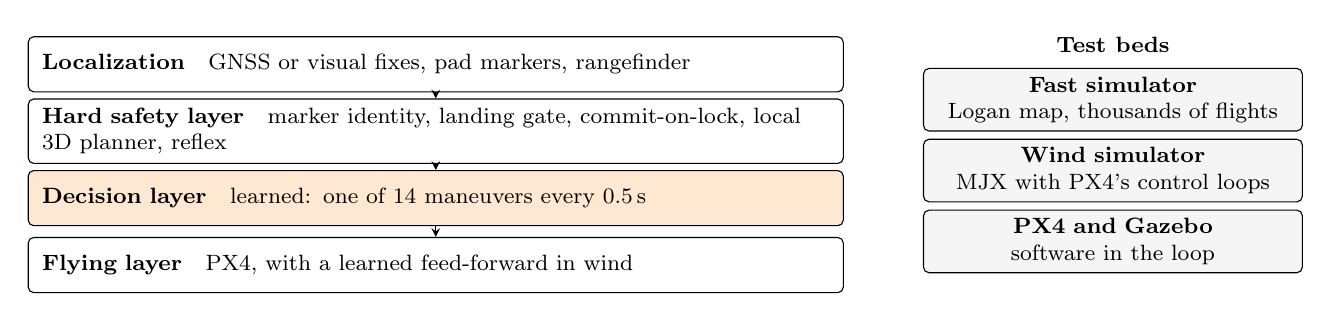
\begin{tikzpicture}[font=\footnotesize, >=stealth,
  layer/.style={draw, rounded corners=2pt, text width=10.0cm, minimum height=7mm, align=left, inner xsep=5pt},
  bed/.style={draw, rounded corners=2pt, text width=4.6cm, minimum height=7mm, align=center, fill=black!4, inner sep=3pt}]
  \node[layer] (loc)  at (0, 0)     {\textbf{Localization}\hspace{1em}GNSS or visual fixes, pad markers, rangefinder};
  \node[layer] (safe) at (0, -0.85) {\textbf{Hard safety layer}\hspace{1em}marker identity, landing gate, commit-on-lock, local 3D planner, reflex};
  \node[layer, fill=orange!18] (dec) at (0, -1.7) {\textbf{Decision layer}\hspace{1em}learned: one of 14 maneuvers every 0.5\,s};
  \node[layer] (fly)  at (0, -2.55) {\textbf{Flying layer}\hspace{1em}PX4, with a learned feed-forward in wind};
  \foreach \a/\b in {loc/safe, safe/dec, dec/fly} \draw[->] (\a.south) -- (\b.north);
  \node[bed] (fast) at (8.6, -0.45) {\textbf{Fast simulator}\\ Logan map, thousands of flights};
  \node[bed] (mjx)  at (8.6, -1.35)  {\textbf{Wind simulator}\\ MJX with PX4's control loops};
  \node[bed] (gz)   at (8.6, -2.25) {\textbf{PX4 and Gazebo}\\ software in the loop};
  \node[font=\footnotesize\bfseries] at (8.6, 0.25) {Test beds};
\end{tikzpicture}
\caption{The landing stack: four layers, one learned decision layer, and the three test beds that run it.}\label{fig:stack}
\end{figure*}


Figure~\ref{fig:stack} shows the stack. Each layer answers one question and hands a smaller problem to the layer below it.

\textbf{Localization.} The drone localizes in two stages (Figure~\ref{fig:pad}(b)). With GNSS available, PX4's estimator (EKF2) fuses it. For the global approach without GNSS, an absolute visual localization module matches the downward camera image against satellite imagery of the suburb. It sends each accepted fix to EKF2 as an auxiliary global position. These fixes are a few meters off, enough to bring the drone to the pad but not to land it.

\textbf{Terminal pad localization.} The delivery pad is a 5~m square mat carrying three ArUco markers \cite{garrido2014} in a row, 1.80, 1.20 and 0.15~m across (Figure~\ref{fig:pad}(a)). The smallest sits at the touchdown point, and the drone reads the largest first and the smallest last. Each readable marker gives a position relative to the pad, and a downward rangefinder gives height. A touchdown error therefore measures this terminal stage, not the satellite-image fixes.

% The delivery pad and the two-stage localization (TikZ), two panels with their labels below. Every size and position is
% make_pad.py's MARKERS and MAT; the radii are the landing tests of gz_learner.py (1.0 m) and wind/gz_windland.py (PAD_R 0.75 m).
\begin{figure*}[t]\centering
\begin{minipage}[b]{0.29\textwidth}\centering
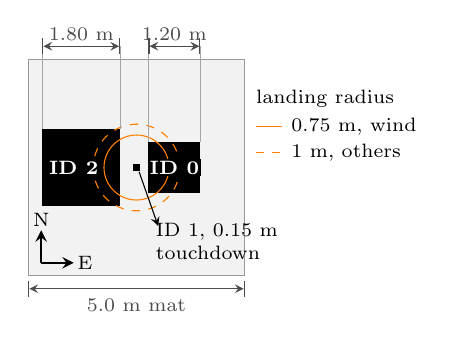
\begin{tikzpicture}[>=stealth, font=\scriptsize, x=0.55cm, y=0.55cm]
  \fill[black!5] (-2.5,-2.5) rectangle (2.5,2.5);
  \draw[black!40] (-2.5,-2.5) rectangle (2.5,2.5);
  \fill (-2.175,-0.9) rectangle (-0.375,0.9);                           % ID 2, 1.80 m, centre x = -1.275
  \fill (0.275,-0.6) rectangle (1.475,0.6);                             % ID 0, 1.20 m, centre x = +0.875
  \fill (-0.075,-0.075) rectangle (0.075,0.075);                        % ID 1, 0.15 m, at the origin
  \draw[orange] (0,0) circle (0.75);
  \draw[orange, dashed] (0,0) circle (1.0);
  \node[white, fill=black, inner sep=0.8pt, font=\scriptsize\bfseries] at (-1.45,0) {ID 2};
  \node[white, fill=black, inner sep=0.8pt, font=\scriptsize\bfseries] at (0.875,0) {ID 0};
  % sizes above the mat, on extension lines from the markers' corners
  \foreach \xa/\xb/\h in {-2.175/-0.375/0.9, 0.275/1.475/0.6} \draw[black!35, very thin] (\xa,\h) -- (\xa,2.8) (\xb,\h) -- (\xb,2.8);
  \draw[|<->|, black!70] (-2.175,2.8) -- node[above=2pt, inner sep=0pt] {1.80 m} (-0.375,2.8);
  \draw[|<->|, black!70] (0.275,2.8) -- node[above=2pt, inner sep=0pt] {1.20 m} (1.475,2.8);
  \draw[->] (0.06,-0.1) -- (0.5,-1.35) node[below right=-2pt, align=left, inner sep=1pt] {ID 1, 0.15 m\\touchdown};
  \draw[->, thick] (-2.2,-2.2) -- (-1.45,-2.2) node[right, inner sep=1pt] {E};
  \draw[->, thick] (-2.2,-2.2) -- (-2.2,-1.45) node[above, inner sep=1pt] {N};
  \draw[|<->|, black!70] (-2.5,-2.8) -- node[below] {5.0 m mat} (2.5,-2.8);
  \node[anchor=west, inner sep=0pt] at (2.75,1.6) {landing radius};
  \draw[orange] (2.75,0.95) -- (3.35,0.95) node[right, black] {0.75 m, wind};
  \draw[orange, dashed] (2.75,0.35) -- (3.35,0.35) node[right, black] {1 m, others};
\end{tikzpicture}\\[3pt]
{\small (a) The pad from above}
\end{minipage}\hfill
\begin{minipage}[b]{0.69\textwidth}\centering
\begin{tikzpicture}[>=stealth, font=\scriptsize, box/.style={draw, rounded corners=1.5pt, text width=2.5cm, align=flush left, inner sep=2pt, minimum height=0.66cm},
                    hd/.style={font=\scriptsize\bfseries, anchor=south west, inner sep=0.5pt}]
  \node[box] (s1) at (0,0.62) {GNSS on, visual fixes begin};
  \node[box, right=0.36cm of s1] (s2) {GNSS off once 4 fixes arrive within 15 s};
  \node[box, right=0.36cm of s2] (s3) {each accepted fix goes to PX4's EKF2};
  \node[box, right=0.36cm of s3] (s4) {over the pad, its markers come into view};
  \node[box] (s5) at (0,-1.0) {pad identity read five times, then commit};
  \node[box, right=0.36cm of s5] (s6) {marker pose across, rangefinder height};
  \node[box, right=0.36cm of s6] (s7) {descent only through the landing gate};
  \node[box, right=0.36cm of s7] (s8) {touchdown scored against Gazebo truth};
  \node[hd] at ([yshift=2pt]s1.north west) {A: global approach on satellite-image fixes, median fix error 2.1 to 2.3 m};
  \node[hd] at ([yshift=2pt]s5.north west) {B: terminal landing on the pad's markers, touchdown within 0.19 m};
  \foreach \a/\b in {1/2, 2/3, 3/4, 5/6, 6/7, 7/8} \draw[->] (s\a) -- (s\b);
  % A to B: down from the last box, back under row A, and in from the left, clear of B's heading
  \draw[->, rounded corners=3pt] (s4.south) -- ++(0,-0.2) -| ([xshift=-0.25cm]s5.west) -- (s5.west);
\end{tikzpicture}\\[3pt]
{\small (b) The two localization stages}
\end{minipage}
\caption{The delivery pad and its two localization stages.}\label{fig:pad}
\end{figure*}


\textbf{Hard safety layer.} Some rules no decider may override, and that is all we mean by hard. The rules act on the same imperfect sensing as the deciders, so they guarantee nothing about a person hidden in fog or a magpie seen late. The drone lands only after it reads the customer's marker identity. Below 6~m it descends only while centered and still over the pad, a condition we call the landing gate. After five reads of its own pad's marker it commits to that pad, a rule we call commit-on-lock. A short loss of sight then means a slow descent at 0.5~m/s instead of a new search. A local 3D planner runs weighted A* over the surveyed map and a voxel map from the forward depth camera. It keeps 2~m from anything blocked and pays a cost for passing within 5~m. Between decisions, a reflex applies the rule's magpie dodge every 0.25~s. The fast simulator flies thousands of drones at once and runs a lighter version of this layer. It checks the map and voxel map ahead instead of running A*. It models no wind and counts any touchdown within 1~m of the pad center, so it has no landing gate.

\textbf{Decision layer.} Every 0.5~s one decider picks one of 14 candidate velocity commands. Two are the rule's command and the guidance command it starts from, which heads for the pad. The guidance command also appears turned $45^\circ$ or $90^\circ$ either way, reversed, at half speed, held level and climbing. The other four are landing anyway, hovering, climbing straight up and flying away from the helipad. Every candidate is capped at 8~m/s across, 3~m/s up and 2.5~m/s down. The rule, both planners and the learner choose from the same list, so any difference between them comes from the decision alone.

\textbf{Flying layer.} PX4 tracks the chosen velocity. In the wind study a flying learner adds an acceleration feed-forward of at most 3~m/s$^2$ per axis to that velocity setpoint.

\subsection{Three Test Beds}

\textbf{Fast simulator.} Thousands of deliveries advance in lock-step on the GPU in 0.25~s steps, with a 300~s limit per flight. The map covers 4~km by 4~km of Logan at 1~m resolution, rebuilt from the 2023 airborne LiDAR survey (Figure~\ref{fig:world}). It holds 1,324 candidate pads and a hospital helipad. Each flight starts 50~m up, at most 1~km from its pad in the direction of the depot. PX4's velocity response enters as first-order lags that we measured on PX4, 0.69~s horizontal and 0.23~s vertical. An air ambulance arrives on half the flights, and in the world we report it always comes from the north-west. Up to six other delivery drones fly between the depot and customers, and people and cars appear near the pad.

We apply three drone safety rules that the Civil Aviation Safety Authority (CASA) sets for recreational flying \cite{casa2026}. They serve as safety constraints in the simulation, not as an assessment of regulatory compliance for commercial delivery. The drone stays below 120~m and at least 30~m from people, and never flies over a person. Within 1.4~km of a helicopter landing site, it moves away from a helicopter that is nearby, taking off or landing. A near mid-air collision (NMAC) with the air ambulance follows ASTM F3442 \cite{astm2023}, which covers encounters with crewed aircraft: 152~m horizontally and 30~m vertically. We assume a 30~m separation between drones, since we found no CASA figure for it. A clean delivery is a touchdown on the right pad with no crash, no NMAC and no rule broken during the flight.

\begin{figure}[t]\centering\includegraphics[width=0.76\linewidth]{world}
\caption{Logan from the 2023 LiDAR survey.}\label{fig:world}\end{figure}

We test four conditions. Clear is the world as described. Unmapped adds tall structures that the survey does not contain, such as cranes, which the drone senses only with its depth camera. Fog covers every flight. We measured in Gazebo how often the drone reads the marker through fog at each height, relative to calm air. The share falls from every frame at 5~m to 36\% of frames at 46~m. Fog hides people as well.

Magpie adds a territorial Australian magpie near half the pads. It attacks from behind, keeps steering through its dive with turns of up to 20~m/s$^2$, and commits to its path 0.3~s before contact. The drone knows the magpie either exactly or through a model of a six-camera rig, its small detector and a tracker, calibrated on Gazebo renders of that rig.

\textbf{Wind simulator.} For wind we need flight dynamics, so we model the x500 quadrotor in MuJoCo \cite{todorov2012}, run with MuJoCo XLA (MJX) on the GPU. The drone is a 2.584~kg rigid body with Gazebo's motor and propeller-drag model. We emulate PX4's velocity, attitude and rate loops and its control allocation with PX4's default gains.

We report the mean wind 10~m above ground as W10. The same wind drives MJX and a Gazebo plugin we wrote: a logarithmic profile, turbulence in the low-altitude form of MIL-F-8785C \cite{milf8785c}, and one-minus-cosine gusts. The specification scales turbulence by the wind at 20~ft, and we scale it by W10. The two simulators agree closely. For a 0 to 8~m/s velocity step, 63\% of the response takes 0.85~s in Gazebo and 0.80~s in MJX. Hovering in a steady 15.8~m/s wind, the drone tilts 22.5$^\circ$ in Gazebo and 22.6$^\circ$ in MJX.

The wind task starts 30~m up and 15 to 25~m from a back-yard pad. A house stands 2.5 to 8~m away, and a tree stands beside the pad in 60\% of yards. A landing counts when the drone touches down within 0.75~m of the center, sinking slower than 1~m/s and sliding slower than 0.5~m/s. Within 0.35~m of the house or tree counts as a crash, any other touchdown as hard or off the pad, and 90~s aloft as a timeout.

\textbf{PX4 and Gazebo.} The last test bed runs PX4 v1.16.2 in software-in-the-loop with Gazebo \cite{koenig2004}. The x500 model carries our camera rig. It has a forward stereo depth camera with a color sensor, wide cameras to the left, right and rear, and a landing camera on a gimbal. One variant adds a wide camera looking up. The suburb, pads, crane and magpie are the fast simulator's, rebuilt as Gazebo worlds.
